\chapter{Grundlagen} 
\label{ch:grundlagen}
In diesem Kapitel möchte ich einige Grundlagen für die weiteren Kapitel dieser Arbeit legen. Zunächst erläutere ich den Aufbau eines neuronalen Netzes im allgemeinen, die Bedeutung von rekurrenten neuronalen Netzen (RNN), zeige am Bouncing Ball Szenario das Vanishing Gradient Problem auf und mache so die Notwendigkeit der LSTM-Technik deutlich.
\section{Neuronale Netze}

\begin{figure}
	\centering
	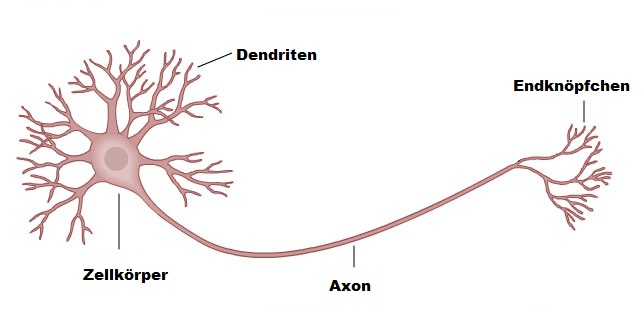
\includegraphics[width=0.7\textwidth, height=130px]{pics/neuron.jpg}	
	\caption{Schematische Darstellung eines biologischen Neuron \cite{bib:neuron}}
	\label{img:neuron}
\end{figure}
\begin{figure}
	\centering
	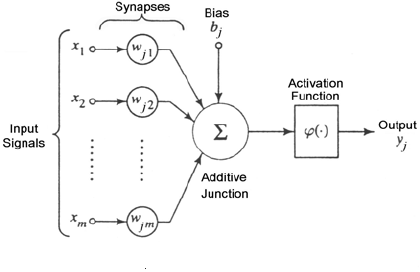
\includegraphics[width=0.7\textwidth, height=130px]{pics/aneuron.png}	
	\caption{Schematische Darstellung einer Möglichkeit, ein künstliches Neuron zu simulieren \cite{bib:aneuron}}
	\label{img:aneuron}
\end{figure}

Als neuronales Netz bezeichnet man eine verwobene Struktur zwischen vielen einzelnen Zellen von meistens gleichem - aber keineswegs darauf beschr\"anktem - Aufbau, den sogenannten Neuronen. Eine solche Zelle hat immer die Eigenschaft, dass sie Signale von anderen Zellen empfängt, diese gewichtet aufakkumuliert und abhängig von einer internen Aktivierungsfunktion ein entsprechendes Signal an andere Zellen weitergibt, die damit ihrerseits diesselbe Prozedur durchlaufen. Ein neuronales Netz im Gehirn einer Ameise hat ca. 250.000 Neuronen, ein menschliches 86 Milliarden \cite{bib:number} und wir haben lediglich eine wage Vorstellung, wozu diese imstande sind. In der Informatik werden solche Strukturen als künstliche neuronale Netze nachgebildet und je nach Problemstellung abgewandelt. Zur Vereinfachung meinen wir ab sofort, sofern nicht explizit anders angegeben, mit neuronalen Netzen künstliche neuronale Netze.
\begin{figure}
	\centering
	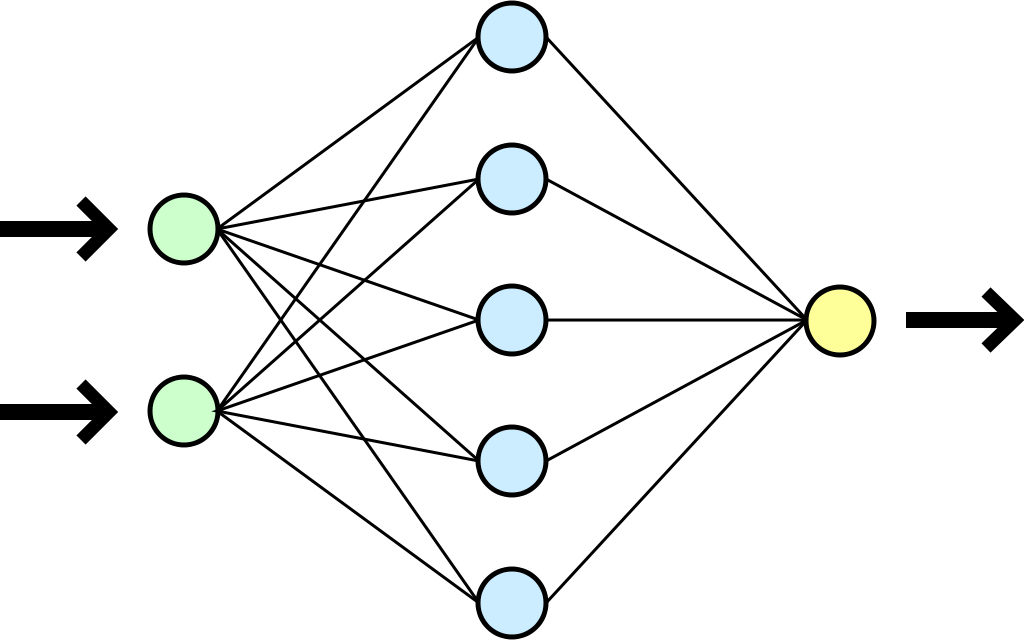
\includegraphics[width=0.7\textwidth, height=130px]{pics/MLP.png}	
	\caption{Ein Multilayer Perceptron mit 2 Inputneuronen(grün), einem Hidden Layer mit 5 Neuronen(blau) und einem einzelnen Outputneuron(gelb).   \cite{bib:mlp}}
	\label{img:mlp}
\end{figure}
Es gibt viele verschiedene Arten von neuronalen Netzen, die einfachste von Ihnen ist das Multilayer Perceptron (MLP). Die Zellen werden zu mehreren Ebenen(Layer) zusammengefügt. Erst das Inputlayer, in das die Daten hineingegeben werden, dann die versteckten Layer, versteckt weil hier wie in einer Blackbox die Berechnungen passieren und dann an das Outputlayer weiterleitet, aus welchem das Ergebnis des Netzes kommt.Es gibt eine geordnete Datenflussrichtung, eine Zelle erhält ihren Input von jeder Zelle der vorigenen Ebene und gibt ihren Output entsprechend an jede Zelle der folgenden Ebene weiter, Feedforward genannt. Ein solches Netz sieht man in Abbildung \ref{img:mlp}.  
\begin{gather}
x_{j} = \varphi_{h}(net_{h}) = \varphi_{h}(\sum_{i=1}^{n} x_{i}w_{ij}) 
\label{eq:act}
\end{gather}
In jeder Zelle \(j\) werden die Inputsignale \(x_{i}\), also die Aktivierungen der vorigen Zellen mit Index \(i\) unterschiedlich gewichtet \(w_{ij}\) aufsummiert \(net_{h}\) (Abbildung \ref{img:aneuron}).  Eben diese Gewichte sind der Kern des maschinellen Lernens, da bei einmal geschickt gefundenen Gewichten, komplexe Aufgabenstellungen und Probleme mit (vergleichsweise) wenig Rechen- sowie Programmieraufwand gelößt werden können. Im Wesentlichen versucht ein MLP immer eine Funktion zu berechnen welches einen Inputvektor der Größe \(n\) auf einen Outputvektor der Größe \(m\) abbildet.
\begin{gather*}
f_{MLP}: R^n \to R^m 
\end{gather*}
Ein Beispiel für eine solche Funktion wäre für ein gegebenes Bild zu entscheiden, ob darauf ein Gesicht zu erkennen ist. Die Länge des Inputs wäre hier z.B. mehrere Millionen, einfach die Pixelwerte, als Output wäre hier nur eine Zahl, nämlich ob ein Gesicht zu sehen ist oder nicht. Der Output \(y\) des Netzes ist also abhängig vom Input \(x\), aber auch von den Gewichten \(w\).
Die Gewichte werden entweder mit Hilfe von Trainingsdaten, bestehend aus Inputdaten und entsprechenden Outputdaten, also den zugehören Lösungen, oder mit einer zu erlenenden Zielfunktion, die einem aus gegebenen Inputdaten die gewünschten Lösungen liefert, über mehrere Trainingsläufe (Epochen) justiert. Fügt man in die Inputebene entsprechende Inputdaten \(x\) ein, berechnet die Aktivierungen aller Zellen, vergleicht die Aktivierungen \(y\) des Outputlayers des Netzes mit den gegebenen Lösungen \(z\) und erhält eine Fehlerabweichung \( E(z,y)\): 
\begin{equation}
E(z,y) =_{def} \dfrac{1}{2} \sum_{i=1}^{m}(z_{i}-y_{i})^{2}
	\label{eq:err}
\end{equation}
Die Herausforderung ist es nun, diejenigen Gewichte \(w\) zu finden, für die die Fehlerabweichung über alle Trainingsdaten minimal ist.
\begin{equation}
arg_{w} min( \sum_{(x,z)\in trainset} E(z,f_{MLP}(w,x)))
\label{eq:err}
\end{equation}
Bei der Anpassung der Gewichte der versteckten Zellen hat man aber das Problem, das man keinen direkten Fehler für sie kennt, da man nur für die Outputschicht den gewünschten Output hat und so einen Fehler ermitteln kann. Als Lösung ist hier der Backpropagation-Algorithmus geläufig. Dieser besteht aus 3 Schritten, die entweder solang durchlaufen werden bis der Fehler einen festgesetzten Schwellenwert(Threshold) unterschreitet, oder eine vorgegebene Anzahl an Epochen durchlaufen wurde. 
\begin{description}	\item[Feedforward]\hfill \\
	Das Inputlayer wird mit der Eingabe des jeweiligen Testsatzes befüllt und die Aktivierungen vorwärts Layer für Layer, Zelle für Zelle berechnet.  
	\item[Backward-Pass]\hfill \\ 
	Das Ergebnis am Outputlayer wird mit der gewünschten Lösung des Testsatzes verglichen und der Fehler berechnet. Diese werden entsprechend gewichtet die unteren Layer rückwärts Zelle für Zelle rückpropagiert. Oft werden hier statt dem tatsächlichen Fehler direkt der Gradient bzw. ein Zwischenwert für dessen Berechnung propagiert\ref{eq:bp}.
	\item[Anpassen der Gewichte]\hfill \\ Dies ist der wichtige Schritt, hier werden nun Zelle für Zelle die Gewichte entsprechend des Gradienten angepasst. Mit den neuen Gewichten ist in der Regel der Output des Netzes genauer, der Fehler also geringer und der Algorithmus lässt die Fehlerfunktion im Idealfall gegen 0 konvergieren.\cite{bib:nn}
\end{description}
Die Gewichte werden anhand eines absteigenden Gradienten der Fehlerfunktion, abgeleitet nach den Gewichten \(w_{ij}\), aktuallisiert.  Hierzu werden die \(\delta\), die aufsummierten Fehler für jede Zelle wie folgt berechnet: 
\begin{gather}
\delta_{k} = \varphi_{k}'(net_{k})(x_{k}-z_{k}) \\
\delta_{h} = \varphi_{h}'(net_{h})\sum_{k\in K}w_{hk}\delta_{k} \mid K Neuronen aus dem oberen Layer 
\label{eq:err}
\end{gather}
Berechnung des Delta Fehlers für jedes Neuron des Outputlayers(oben) und der versteckten Layer (unten). \\
Wobei erst für die Outputlayer die \(\delta_{k}\) gebildet und in die jeweils unteren Layer beim bilden der \(\delta_{h}\) gewichtet aufsummiert (Backpropagation). Die Formel für das Gewichtsupdate mit einer Lernrate \(\eta\) lautet dann:
\begin{gather}	
	\Delta w_{ij} =_{def}  -\eta \frac{\partial E}{\partial w_{ij}} = -\eta x_{i}\delta_{j}  
\end{gather} 
Formel zur Berechnung der Gewichtupdates aus dem Gradienten der Fehlerfunktion \cite{bib:bp}\\
Es gibt nun noch verschiedene Techniken um das Ergebnis weiter zu verbessern und das lernen noch schneller und stabiler zu machen, an dieser Stelle wollen wir unser Augenmerk aber in eine andere Richtung lenken. 
\section{Rekurrente Neuronale Netze}

Neuronale Netzwerke haben einen für einen 1-Dimensionalen Inputvektor einen eindeutig zu berechnenden 1-Dimensionalen Outputvektor und für die meisten Problemstellungen ist auch genau diese Kompetenz gefordert. Es gibt aber auch Probleme, bei denen der Output nicht nur von diesem, sondern auch von allen beziehungsweise einigen vorigen Inputs und Zuständen abhängt. Ein anschauliches Beispiel wäre hier die Klassifizierung von Videoausschnitten, wo die Bedeutung eines einzelnen Frames vom Kontext der vorigen Frames abhängt, hingegen ein einfacheres Beispiel wäre das in dieser Arbeit betrachtete Bouncing Ball Szenario. Befindet sich ein Ball im Punkt \(p_{1}=(0/0)\) und der nächste Ort \(p_{2}\) soll vorhergesagt werden, ist es natürlich entscheidend ob der Ball sich zuvor beispielsweise im Punkt \(p_{0}=(0.1/0,1)\) oder im Punkt \(p_{0}=(-0.1/-0.1)\) befand. Hierzu werden den Zellen aus dem verstecktem Layer des neuronalen Netzes rekurrente (lat. recurrere:zurücklaufen) Verbindungen hinzugefügt.
\begin{figure}
	\centering
	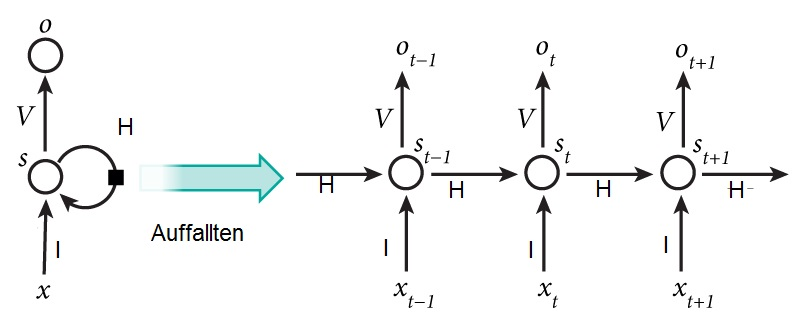
\includegraphics[width=0.7\textwidth, height=130px]{pics/rnn.jpg}	
	\caption{Um Backpropagation für ein rekurrentes Netz zu benutzen, muss man es durch die Zeit auffallten. \cite{bib:rnn}}
	\label{img:rnn}
\end{figure}
Eine Zelle \textit{h} bekommt nun im Zeitpunkt \textit{t} seinen Input immernoch von allen Zellen des unteren Layers \textit{I}, zusätzlich nimmt sie aber auch noch als Input den Output aller Zellen desselben Layers, aber aus dem vorigen Zeitschritt \textit{H'}, die Formel für die Aktivierung lautet also: 
\begin{gather}
x^{t}_{h}=\varphi_{h}(net_{h}^{t})=\varphi_{h}(\sum_{i \in I}w_{ih}x^{t}_{i}+\sum_{i \in H'}w_{h'h}x^{t-1}_{h'})
\end{gather}

Da diese neuen rekurrenten Inputs auch wieder gewichtet verarbeitet werden, müssen diese erst noch geschickt gefunden werden. Dies macht man mit Backpropagation durch die Zeit (BPTT). Dies passiert analog zur Backpropagation im MLP, jedoch werden die einzelnen Zeitschritte aufgeklappt (Abbildung \ref{img:rnn}). Die Backpropagation berechnet sich also wiefolgt:
\begin{gather}
	\delta_{k}^{t} = \varphi_{k}'(net_{k}^{t})(x_{k}^{t}-z^{t}_{k}) \\
	\delta_{h}^{t} = \varphi_{h}'(net_{h}^{t})(\sum_{k \in K}w_{hk}\delta^{t}_{k}+\sum_{h' \in H'}w_{hh'}\delta^{t+1}_{h'})
\end{gather}
Berechnung des Delta Fehlers für jedes Neuron des Outputlayers(oben) und der versteckten Layer (unten). \\ \cite{bib:rnn}
Den Backpropagation Algorithmus wie bei einem Multilayer Perzeptron anwenden um das Netz zu trainieren und passende Gewichte, auch für die rekurrenten Verbindungen zu erhalten. Nun hat man ein Neuronales Netz mit einer Art Kurzzeitgedächtnis, welches beim Auswerten des Inputs die Nahe Vergangenheit mit in Betracht zieht. Hat es in der Anwendung aber tiefere Abhängigkeiten, wo ein vergangener Input einen Einfluss auf die fernere Zukunft hat, hat auch das RNN noch Schwierigkeiten: 
\section{Das Vanishing Gradient Problem}
\begin{figure}
	\centering
	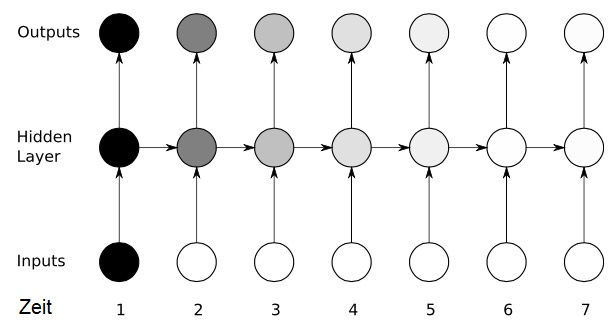
\includegraphics[width=0.7\textwidth, height=130px]{pics/vgp.jpg}	
	\caption{Das Problem vom verschwindendem Gradienten in einem rekurrenten Netz. Ein Fehler im Zeitschritt 1 erzeugt einen Gradienten, der aber auf die folgenden Zeitschritte immer weniger Einfluss hat.\cite{bib:vgp}}
	\label{img:vgp}
\end{figure}
Wir haben gesehen wie beim Training eines rekurrenten Netzes über die Bildung des Gradienten geschickt Gewichte gefunden werden, die Probleme lösen können bei denen Abhängigkeiten über die Zeit auftreten. Erstrecken sich diese Abhängigkeiten aber über zu große Zeitraume, tritt das Problem vom verschwindendem Gradienten auf. Ein Fehler zum Zeitpunkt \textit{t} erzeugt einen Gradienten der auch Einfluss auf Fehlerberechnung zu den kommenden Zeitpunkte hat, 